
\section{Single Page Application}
\label{sec:Single Page App}

Un single-page application (SPA), o aplicación de página única es una aplicación web o es un sitio web que cabe en una sola página con el propósito de dar una experiencia más fluida a los usuarios como una aplicación de escritorio. \cite{spa_wiki}\\

Una Aplicación de Página Única es básicamente la combinación de AJAX y HTML5 para crear una aplicación web fluida que no necesite recargar la página, esto significa que el trabajo sucede en lado del cliente, es decir en el browser, por lo tanto es necesario de un gran conocimiento de JavaScript, pero actualmente existen Frameworks diseñados para resolver los problemas de manejar JavaScript en diferentes tipos y versiones de navegadores. \emph{Ember.js} es un framework con el cual se puede construir Aplicaciones de Página Única. \\


% SPAs use AJAX and HTML5 to create fluid and responsive Web apps, without constant page reloads. However, this means much of the work happens on the client side, in JavaScript. For the traditional ASP.NET developer, it can be difficult to make the leap. Luckily, there are many open source JavaScript frameworks that make it easier to create SPAs.

% In this article, I’ll walk through creating a simple SPA app. Along the way, I’ll introduce some fundamental concepts for building SPAs, including the Model-View-Controller (MVC) and Model-View-ViewModel (MVVM) patterns, data binding and routing.

% Background

En una aplicación web tradicional cada vez que la aplicación hace una petición al servidor, este renderiza una nueva página HTML la cual es desplegada en el navegador.\\

% In a traditional Web app, every time the app calls the server, the server renders a new HTML page. This triggers a page refresh in the browser. If you’ve ever written a Web Forms application or PHP application, this page lifecycle should look familiar.

%  imagen de este proceso

En una Aplicación de Página Única, después que la primera página es cargada en el navegador, todas las demás interacciones del usuario con la aplicación, generan peticiones AJAX al servidor, las cuales retornan datos, generalmente en formato JSON, de esta forma actualiza porciones de la página con información nueva del servidor, sin recargar la pagina gracias a JavaScript. Esto obliga que la lógica de la aplicación con la que el usuario interactúa se cargue en la primera y única vez que la aplicación es cargada, evitando con esto la molestia de ver como se recarga la página con cada interacción del usuario con la aplicación, la cual se siente fluida y lo más parecida a una aplicación de escritorio que una aplicación web puede llegar a ser.\\



% In an SPA, after the first page loads, all interaction with the server happens through AJAX calls. These AJAX calls return data—not markup—usually in JSON format. The app uses the JSON data to update the page dynamically, without reloading the page. Figure 2 illustrates the difference between the two approaches.

% // image

% Los beneficios de crear un SPA son: La aplicación es más fluida, no existe la molestia de ver que la pagina se recargue a cada rato,
%
% \subsection{Arquitectura de un SPA}
% \label{sub:Arquitectura de un SPA}

En una aplicación de página única, las interacciones del usuario con la aplicación se desarrollan en el navegador y el servidor se encarga de manejar la información, en esta arquitectura se puede observar una separación lógica entre la capa de la presentación de la aplicación y el modelo de negocio o la lógica de la aplicación. Es básicamente una implementación del Patrón de Diseño \emph{MVC}.\\


\subsection{MVC} % (fold)
\label{sub:mvc}
  MVC (Modelo Vista  Controlador) es un patrón arquitectónico que separa
  los datos de la aplicación en la interfaz del usuario y  la lógica del
  negocio, en tres partes cada uno especializado para su tarea, la vista
  maneja lo que es la interfaz del usuario, puede ser gráficamente o solo texto,
  el controlador interpreta las entradas del teclado, mouse, o los cambios
  de la vista de la mejor forma posible y finalmente el modelo maneja el comportamiento
  de los datos de la aplicación.\cite{steveburbeck1992}\\

  Este concepto se desarrolló en 1979 por Trygve Reenskaug el cual da una
  solución al problema de separar la lógica del negocio de la lógica de la presentación.\\
  % al final cada acción o concepto se desarrolla en un lugar determinado.\\
  % los objetivos/resultados/conclusión/facilidades

  % Rails está construido sobre el patrón MVC, esto significa que para cada   pieza de código existe un lugar predeterminado y todas las piezas de código de la aplicación interactúan de forma predeterminada.

  % \begin{description}
    \textbf{Modelo:} Representa la información o los datos y contiene las reglas o métodos para manipular estos datos.     % En la aplicación se utilizó \emph{Bookshelf.js} para interactuar con la base de datos \emph{PostgreSQL}.
    %
    % En el caso de Rails, los modelos son usados principalmente para manejar la interacción con las
    % tablas de la Base de Datos, en la que cada tabla corresponde a un modelo en la aplicaci\'on, para nombrar a estos modelos existe una simple convención que es la de nombrar  a la tabla en forma plural, mientras que el modelo tiene el nombre en singular.
    %
    El Modelo es el principal encargado de manejar  la \emph{lógica del negocio}.

    \textbf{Vista:}  Representa la interfaz de la aplicación.

    % En Rails las vistas  archivos HTML con código Ruby embebido\footnote{ ERB (Embedded Ruby) } que realiza la tarea de representar  datos. Las Vistas son las que generan los datos que son enviados al    navegador web.%browser.

    \textbf{Controlador:} Es el encargado de interactuar entre el modelo y la vista, procesando los datos enviados en el request del navegador web,
    llamando a métodos del modelo para conseguir  \emph{información} de la base de datos,
    posteriormente el controlador envía esta \emph{información} a la vista.
    El Controlador y la Vista son los los encargados de manejar  la \emph{lógica de la presentación}.
  \end{description}


% One benefit of SPAs is obvious: Applications are more fluid and responsive, without the jarring effect of reloading and re-rendering the page. Another benefit might be less obvious and it concerns how you architect a Web app. Sending the app data as JSON creates a separation between the presentation (HTML markup) and application logic (AJAX requests plus JSON responses).

Esta separación hace que diseñar cada capa de la aplicación como un ente distinto, sea sencillo. En una aplicación de página única bien diseñada, es posible cambiar o rediseñar la vista o la presentación de la aplicación sin tocar la implementación de la lógica de la aplicación y viceversa.\\

La arquitectura de un SPA, como se puede ver en la figura \ref{fig:spa_arch}, el \emph{DOM} (\emph{Document Object Model}, es la estructura básica de la página desplegada en el navegador.) de \textbf{solo escritura}, ya que no tiene estado o datos almacenados,cuando la página contiene estado o comúnmente la sesión del usuario, es necesario contener y propagar esta \emph{sesión} por las páginas de la aplicación, generalmente son usados los \emph{cookies} pero cuando la aplicación se compleja y contiene diferentes niveles de permisos, el manejo de esta informacion se complica, por lo que en vez de guardar la información en objetos aleatorios dentro del DOM es necesario una capa de la aplicación donde esté representado objetos definidos toda la información y el estado de la aplicación, el cual es el \emph{Modelo}, esta capa también es la encargada guardar y/o extraer los datos del \emph{Storage}, que dependiendo de la aplicación puede ser una base de datos o el mismo navegador, \emph{localStorage} es una implementación de HTML5 que permite almacenar información en objetos JSON en el Navegador, la \emph{Vista} o \emph{View} se encarga de observar lo cambios ocurridos en el \emph{Modelo} y reflejar estos cambios en el \emph{DOM}, el cual es una renderización de un \emph{Template}.\\

\begin{figure}[H]
  \begin{center}
    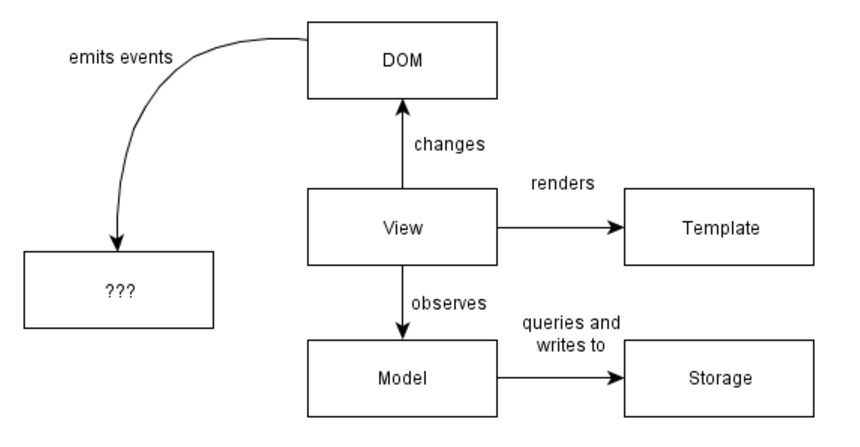
\includegraphics[width=0.9\textwidth]{spa_arch}
    \caption[SPA Architecture ]{Arquitectura de una Aplicación Web Moderna}
    \label{fig:spa_arch}
    \caption*{Fuente: \cite{xp_addison} }
  \end{center}
\end{figure}


Como se puede observar en la figura \ref{fig:spa_arch}, la arquitectura de un SPA es claramente  una implementación del patrón arquitectónico MVC, que en este caso en \emph{Controlador} como una capa específica está desapareciendo, por esa razón no aparece en el diagrama, porque cuando existe algún cambio en el \emph{DOM}, este cambio también se registra en la \emph{Vista} y ya que el \emph{Modelo} tiene el control de la información, la implementación de la lógica del negocio se puede repartir entre estas 2 capas. El patrón arquitectónico MVC no es inmutable y se lo puede implementar dependiendo del tipo de aplicación.\\

% En \emph{Ember.JS} según a la versión también la lógica del negocio es implementada


En la arquitectura de un SPA la lógica de la aplicación es implementada, generalmente y en el presente proyecto, en un API y la capa de la presentación al estar en el navegador es implementada con una combinación de HTML, CSS y JavaScript, lo cual es bastante complejo, pero gracias a frameworks como ser \emph{Backbone.JS}, \emph{AngularJS}, \emph{EmberJS}, etc. Los cuales agilizan en gran medida la implementación de una aplicación de página única.\\




% This separation makes it easier to design and evolve each layer. In a well-architected SPA, you can change the HTML markup without touching the code that implements the application logic (at least, that’s the ideal). You’ll see this in action when I discuss data binding later.



% In a pure SPA, all UI interaction occurs on the client side, through JavaScript and CSS. After the initial page load, the server acts purely as a service layer. The client just needs to know what HTTP requests to send. It doesn’t care how the server implements things on the back end.

% With this architecture, the client and the service are independent. You could replace the entire back end that runs the service, and as long as you don’t change the API, you won’t break the client. The reverse is also true—you can replace the entire client app without changing the service layer. For example, you might write a native mobile client that consumes the service.
%
%
%
% The MVC and MVVM Patterns
%
% The MVC pattern dates back to the 1980s and early graphical UIs. The goal of MVC is to factor the code into three separate responsibilities, shown in Figure 7. Here’s what they do:
%
% The model represents the domain data and business logic.
% The view displays the model.
% The controller receives user input and updates the model.

% // mvc image
